% Springer LNCS format (llncs class v2.26, from CTAN).
% Numbers and tables come from generated/ -- run `python src/make_paper_tables.py`
% from the repository root to refresh them. Do not type result numbers by hand.
\documentclass[runningheads]{llncs}

\usepackage[T1]{fontenc}
\usepackage{graphicx}
\usepackage{xcolor}

% Generated by src/make_paper_tables.py -- do not edit by hand.
\newcommand{\RawRows}{1{,}048{,}575}
\newcommand{\RawColumns}{27}
\newcommand{\Events}{496{,}042}
\newcommand{\MultiCopyEvents}{466{,}466}
\newcommand{\MaxCopies}{14}
\newcommand{\DelayConflictEvents}{30}
\newcommand{\DateMin}{31 January 2022}
\newcommand{\DateMax}{26 August 2023}
\newcommand{\DistinctDates}{417}
\newcommand{\NRoutes}{9}
\newcommand{\NTrips}{75{,}781}
\newcommand{\NStops}{50}
\newcommand{\NVehicles}{36}
\newcommand{\WinsorLow}{$-$206}
\newcommand{\WinsorHigh}{508}
\newcommand{\RawDelayMax}{44{,}575}
\newcommand{\ClippedLow}{4{,}987}
\newcommand{\ClippedHigh}{4{,}815}
\newcommand{\TargetMean}{66.1}
\newcommand{\TargetStd}{121.2}
\newcommand{\MissingStopEvents}{11}
\newcommand{\CutoffDate}{31 July 2023}
\newcommand{\EventsAfterCutoff}{9{,}389}
\newcommand{\TimeTrainRows}{372{,}460}
\newcommand{\TimeTrainDates}{320}
\newcommand{\TimeTrainLast}{12 May 2023}
\newcommand{\TimeTestFirst}{13 May 2023}
\newcommand{\TimeTestDates}{80}
\newcommand{\TimeTestPeriodRows}{114{,}193}
\newcommand{\FixedTestCap}{20{,}000}
\newcommand{\FewshotTestCap}{2{,}000}
\newcommand{\FewshotSeeds}{3}
\newcommand{\FewshotTabpfnRuns}{243}
\newcommand{\TripSeeds}{5}


% Visible marker for anything still to be written or confirmed.
\newcommand{\todo}[1]{\textcolor{red}{[TODO: #1]}}

\begin{document}

\title{\todo{Title, to be confirmed with the framing. Working title: Predicting
Ferry Arrival Delays on Routes with Little or No History}}

\titlerunning{\todo{Short title}}

\author{\todo{Author names}}
\authorrunning{\todo{Author running head}}
\institute{\todo{Affiliation and e-mail addresses}}

\maketitle

\begin{abstract}
\todo{Abstract (150--250 words). Placeholder until the framing is confirmed.}

\keywords{\todo{Keywords, separated by} \and \todo{and}}
\end{abstract}

% ---------------------------------------------------------------------------
\section{Introduction}
\todo{Placeholder until the framing is confirmed. Paper question: how well do
tabular models predict delays on ferry routes with little or no history (cold
start), and how does the evaluation split change the conclusions?}

% ---------------------------------------------------------------------------
\section{Related Work}
\todo{To be written. Every reference must be verified before it is added to
\texttt{references.bib}. Topics to cover: delay prediction in public transport;
gradient-boosted trees for tabular data; tabular foundation models; evaluation
under distribution shift and grouped or temporal splits; cold-start and
few-shot prediction.}

% ---------------------------------------------------------------------------
\section{Data and Preprocessing}
\label{sec:data}

\subsection{Source}
The dataset contains stop-level arrival records for Sydney Ferries, each joined
with the weather reading for the departure hour. \todo{State the provenance of
the ferry records and of the weather readings, and who compiled the file.} The
file has \RawRows{} rows and \RawColumns{} columns. Each row gives the trip, the
route, the scheduled start time and date, the position of the stop within the
trip, the stop, the vessel, the arrival delay in seconds (positive when late),
and the weather: dew point, humidity, wind direction, wind speed, pressure and a
text condition.

\subsection{De-duplication}
One ferry event, identified by trip, start date, stop sequence and stop, can
appear on several rows, because an hour can carry more than one weather
reading. Of the \Events{} distinct events, \MultiCopyEvents{} appear more than
once, up to \MaxCopies{} times. The copies of an event differ almost only in
the weather columns; the arrival delay differs between copies in
\DelayConflictEvents{} events. We keep one row per event, with the mean of the
four numeric weather columns and the first copy's value for every other
column. All experiments use these \Events{} events.

The events cover \NRoutes{} routes, \NTrips{} trips, \NStops{} stops and
\NVehicles{} vessels, on \DistinctDates{} dates between \DateMin{} and
\DateMax{}. There are no records for May, June and July 2022.
Table~\ref{tab:routes} gives the size of each route. The routes differ in
size, in the number of stops per trip, and in their typical delay.

\begin{table}[t]
\caption{Events, trips and stops per route after de-duplication. Delay
statistics are computed after clipping (Sect.~\ref{sec:cleaning}).}
\label{tab:routes}
\centering
\small
\setlength{\tabcolsep}{4pt}
% Generated by src/make_paper_tables.py -- do not edit by hand.
\begin{tabular}{lrrrrrrr}
\hline
Route & Events & Share (\%) & Trip ids & Stops & Events/trip id & Mean delay (s) & Std (s) \\
\hline
F1 & 28{,}090 & 5.7 & 14{,}681 & 6 & 1.9 & $-$31.8 & 132.7 \\
F2 & 15{,}140 & 3.1 & 7{,}247 & 8 & 2.1 & 6.4 & 104.2 \\
F3 & 202{,}667 & 40.9 & 13{,}111 & 27 & 15.5 & 65.8 & 113.1 \\
F4 & 94{,}722 & 19.1 & 12{,}194 & 16 & 7.8 & 101.5 & 134.9 \\
F5 & 34{,}201 & 6.9 & 6{,}025 & 10 & 5.7 & 73.4 & 109.3 \\
F6 & 42{,}623 & 8.6 & 5{,}947 & 10 & 7.2 & 39.7 & 89.3 \\
F7 & 11{,}298 & 2.3 & 4{,}088 & 8 & 2.8 & 41.7 & 117.8 \\
F8 & 46{,}591 & 9.4 & 5{,}076 & 15 & 9.2 & 96.2 & 114.0 \\
F9 & 20{,}710 & 4.2 & 7{,}412 & 7 & 2.8 & 71.6 & 117.1 \\
\hline
All & 496{,}042 & 100.0 & 75{,}781 & & & & \\
\hline
\end{tabular}

\end{table}

\subsection{Cleaning and Target}
\label{sec:cleaning}
Weather values stored as text with units are converted to numbers. The start
time is expressed in minutes after midnight. The raw arrival delay has extreme
values, up to \RawDelayMax{}~s, so it is clipped to the interval
[\WinsorLow{}, \WinsorHigh{}]~s, the 1st and 99th percentiles of the raw
values. This changes \ClippedLow{} events at the lower end and \ClippedHigh{}
at the upper end. After clipping, the target has mean \TargetMean{}~s and
standard deviation \TargetStd{}~s.

Missing values are not imputed for the tree-based models and TabPFN. Three
indicator features record whether the stop, the wind direction or the weather
condition is missing; a missing wind direction or condition becomes its own
category. The stop is missing in \MissingStopEvents{} events.

\subsection{Features}
The models use 21 features: six categorical (route, stop, vessel, wind
direction, weather condition, vessel class), twelve numeric (start time, days
since the first date, month, day of year, day of week, stop sequence, dew
point, humidity, wind speed, pressure, seating capacity, and a binary calendar
flag named \texttt{Holidays} in the file) and the three missing-value
indicators. \todo{Confirm the meaning of the \texttt{Holidays} flag with the
data provider: it equals 1 on about 70\% of dates, so it may mark ordinary
days rather than holidays.} The trip identifier is used only to form splits.

Five columns of the file are not used. Precipitation is constant. The hour
duplicates the start time. Wind gust is zero on most rows. Total capacity is
fixed per vessel and closely follows seating capacity. Ridership is a monthly
total per route, which would not be known when a prediction is made.

% ---------------------------------------------------------------------------
\section{Evaluation Protocol}
\label{sec:protocol}

\subsection{Models}
We compare XGBoost~\cite{chen2016xgboost}, LightGBM~\cite{ke2017lightgbm} and
TabPFN~\cite{hollmann2025tabpfn}. \todo{State which TabPFN model version the
hosted API served; the experiments used tabpfn-client 0.4.1.} No
hyperparameter is tuned for any model. XGBoost and LightGBM use the same fixed
settings in every experiment: 300 trees, learning rate 0.1, row and column
subsampling of 0.9, and a maximum depth of 6 (XGBoost) or 31 leaves
(LightGBM). TabPFN is used through its hosted API with default settings.
Categorical features are ordinal-encoded for these three models, and a
category not seen in training receives a separate code.

\paragraph{Training rows given to TabPFN.}
In all experiments TabPFN receives at most 10{,}000 training rows. When the
training set is larger, a uniform random sample of 10{,}000 rows is used.
XGBoost and LightGBM use every training row. To separate the effect of the
model from the effect of the amount of data, we also train XGBoost and
LightGBM on exactly the 10{,}000 rows that TabPFN receives. We refer to this
as the equal-data comparison.

\subsection{Baselines}
Four baselines use statistics of the training rows only:
(a)~the mean delay of all training rows;
(b)~the mean delay per stop;
(c)~the mean delay per route and stop, falling back to (b) for a route and
stop pair not seen in training, and to (a) for a stop not seen in training;
(d)~Ridge regression~\cite{pedregosa2011scikit} with default regularisation on
one-hot encoded categorical features and standardised numeric features, with
missing numeric values replaced by the training median.

\subsection{Splits}
We evaluate under four splits of the same events.
\begin{description}
\item[Random.] 80\% of events for training and 20\% for testing, chosen at
random. Stops of the same trip can fall on both sides.
\item[Trip-grouped.] 80\% of trips for training and 20\% for testing, so that
no trip is on both sides. Repeated with \TripSeeds{} random seeds.
\item[Unseen routes.] Two of the nine routes are held out for testing and the
other seven are used for training. Repeated for five random choices of the
held-out routes.
\item[Time.] Training on the earliest 80\% of calendar dates and testing on the
latest 20\%, with no date on both sides. Events after \CutoffDate{} are removed
for this split only (\EventsAfterCutoff{} events), because the file contains
later records for a single route and the test period should cover all nine.
This leaves \TimeTrainRows{} training events on \TimeTrainDates{} dates up to
\TimeTrainLast{}, and a test period of \TimeTestDates{} dates from
\TimeTestFirst{} to \CutoffDate{}. The split is deterministic.
\end{description}

On the random, trip-grouped and unseen-route splits, models are scored on the
full test set. On the time split, every model is scored on the same fixed
random sample of \FixedTestCap{} of the \TimeTestPeriodRows{} test-period
events. On the time split TabPFN is run on five different random
10{,}000-row samples of the training events; XGBoost and LightGBM are run once
on all training events and once on each of the five samples.

\subsection{Few-Shot Route Experiment}
\label{sec:fewshot-protocol}
This experiment measures how accuracy on a new route grows with the number of
events observed on it. Each of the nine routes in turn is treated as the new
route. Its trips are divided into an adaptation pool (80\% of trips) and a
test set (20\% of trips); the test set is a fixed sample of \FewshotTestCap{}
events, the same for every model and setting.

For $k \in \{0, 100, 500, 1000, 5000\}$, we draw $k$ events from the
adaptation pool trip by trip: whole trips are added in random order, and the
last trip is cut after its first stops so that exactly $k$ events are used. A
new route would be observed in this way, one trip at a time. Because routes
differ in stops per trip, a given $k$ corresponds to different numbers of
trips on different routes. Each setting is repeated with \FewshotSeeds{}
random draws.

Models are trained under two conditions:
\begin{description}
\item[Pooled.] All events of the other eight routes, plus the $k$ events of
the new route. With $k=0$ the model has never seen the new route.
\item[Target-only.] The $k$ events of the new route alone ($k>0$).
\end{description}
In the pooled condition the training set always exceeds 10{,}000 rows. TabPFN
then receives all $k$ events of the new route and a random sample of events
from the other routes, 10{,}000 rows in total. For the equal-data comparison,
XGBoost and LightGBM are also trained on exactly these rows. The four
baselines are evaluated at every $k$ under both conditions.

\subsection{Metrics}
We report the coefficient of determination ($R^2$), the root mean squared
error (RMSE) and the mean absolute error (MAE), the last two in seconds.
$R^2$ is computed on the test set at hand, so a value below zero means that
the model is worse than predicting the mean delay of that test set. Where a
setting is repeated, we report the mean and the standard deviation over the
repetitions.

% ---------------------------------------------------------------------------
\section{Results}
\label{sec:results}
\todo{Prose to be written once the Stage 4 summary and the framing are
confirmed. The tables and the figure below are generated from the results
files.}

\subsection{Effect of the Evaluation Split}
\todo{Text.}

\begin{table}[t]
\caption{$R^2$ by model and evaluation split (mean $\pm$ standard deviation
where a setting is repeated). ``10{,}000 rows'': trained on exactly the rows
TabPFN receives. A dash marks a combination that was not run.}
\label{tab:splits}
\centering
\small
\setlength{\tabcolsep}{4pt}
% Generated by src/make_paper_tables.py -- do not edit by hand.
\begin{tabular}{lrrrr}
\hline
Model & Random & Trip-grouped & Time & Unseen routes \\
\hline
Global mean & -- & 0.000 $\pm$ 0.000 & $-$0.003 & $-$0.028 $\pm$ 0.036 \\
Stop mean & -- & 0.111 $\pm$ 0.005 & 0.137 & $-$0.032 $\pm$ 0.038 \\
Route $\times$ stop mean & -- & 0.131 $\pm$ 0.005 & 0.156 & $-$0.032 $\pm$ 0.038 \\
Ridge & -- & 0.164 $\pm$ 0.005 & 0.173 & $-$0.029 $\pm$ 0.054 \\
\hline
XGBoost, all rows & 0.399 & 0.365 $\pm$ 0.005 & 0.311 & $-$0.398 $\pm$ 0.336 \\
LightGBM, all rows & 0.382 & 0.355 $\pm$ 0.007 & 0.319 & $-$0.420 $\pm$ 0.382 \\
\hline
XGBoost, 10{,}000 rows & -- & 0.226 $\pm$ 0.005 & 0.171 $\pm$ 0.012 & -- \\
LightGBM, 10{,}000 rows & -- & 0.240 $\pm$ 0.008 & 0.211 $\pm$ 0.020 & -- \\
TabPFN, 10{,}000 rows & 0.337 & 0.327 $\pm$ 0.005 & 0.333 $\pm$ 0.005 & 0.000 $\pm$ 0.071 \\
\hline
\end{tabular}

\end{table}

\subsection{Routes with Little or No History}
\todo{Text.}

\begin{figure}[t]
\centering
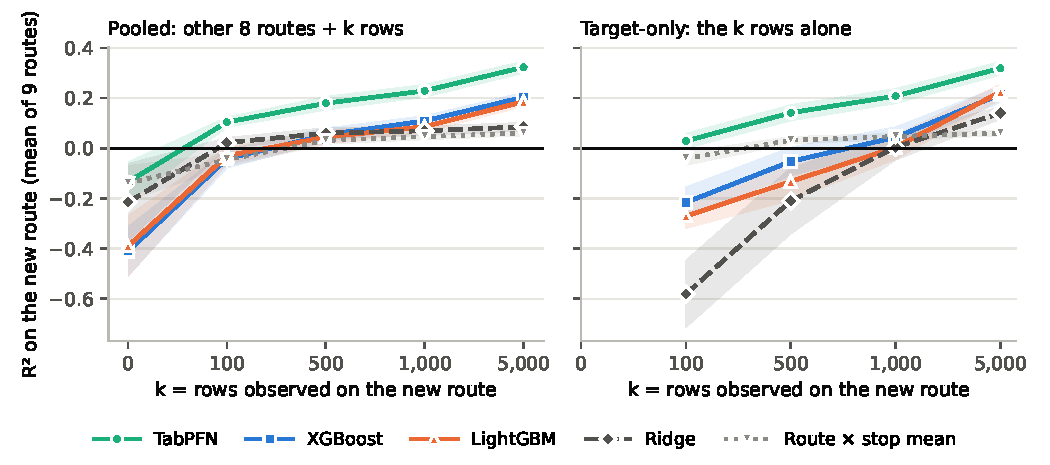
\includegraphics[width=\textwidth]{../figures/6_fewshot_r2_vs_k.pdf}
\caption{$R^2$ on a new route against the number $k$ of events observed on it,
averaged over the nine routes and three draws. Bands show $\pm 1$ standard
error across routes.}
\label{fig:fewshot}
\end{figure}

\begin{table}[t]
\caption{Few-shot route experiment: mean $R^2$ on the new route over the nine
routes and three draws.}
\label{tab:fewshot}
\centering
\small
% Generated by src/make_paper_tables.py -- do not edit by hand.
\begin{tabular}{lrrrrr}
\hline
Model & $k=0$ & $k=100$ & $k=500$ & $k=1{,}000$ & $k=5{,}000$ \\
\hline
\multicolumn{6}{l}{\emph{Pooled (other 8 routes + $k$ rows)}} \\
XGBoost & $-$0.411 & $-$0.042 & 0.053 & 0.109 & 0.204 \\
LightGBM & $-$0.390 & $-$0.030 & 0.044 & 0.086 & 0.186 \\
TabPFN & $-$0.135 & 0.104 & 0.180 & 0.229 & 0.324 \\
Ridge & $-$0.215 & 0.022 & 0.060 & 0.070 & 0.086 \\
Route $\times$ stop mean & $-$0.140 & $-$0.045 & 0.031 & 0.047 & 0.061 \\
Global mean & $-$0.158 & $-$0.158 & $-$0.157 & $-$0.157 & $-$0.154 \\
\hline
\multicolumn{6}{l}{\emph{Pooled, TabPFN's 10{,}000 rows}} \\
XGBoost & $-$0.446 & $-$0.037 & 0.079 & 0.136 & 0.256 \\
LightGBM & $-$0.460 & $-$0.033 & 0.095 & 0.149 & 0.257 \\
\hline
\multicolumn{6}{l}{\emph{Target-only ($k$ rows)}} \\
XGBoost & -- & $-$0.216 & $-$0.053 & 0.044 & 0.215 \\
LightGBM & -- & $-$0.270 & $-$0.133 & 0.003 & 0.225 \\
TabPFN & -- & 0.029 & 0.142 & 0.208 & 0.319 \\
Ridge & -- & $-$0.581 & $-$0.210 & 0.004 & 0.141 \\
Route $\times$ stop mean & -- & $-$0.041 & 0.032 & 0.047 & 0.061 \\
Global mean & -- & $-$0.021 & $-$0.007 & $-$0.004 & $-$0.002 \\
\hline
\end{tabular}

\end{table}

\todo{Decide whether the per-route table
(\texttt{generated/tab\_fewshot\_routes.tex}) and the RMSE table
(\texttt{generated/tab\_splits\_rmse.tex}) fit within the page limit.}

% ---------------------------------------------------------------------------
\section{Limitations}
\label{sec:limitations}

\paragraph{The source file may be incomplete.}
The file has \RawRows{} rows, which is the row limit of a spreadsheet
application, and its last month contains records for one route only. It was
probably truncated when it was exported. \todo{Confirm with the data provider
whether the file is complete.} The records after \CutoffDate{} are excluded
from the time split for this reason, and there are no records for three months
of 2022.

\paragraph{Weather is observed, not forecast.}
The weather features are the readings for the departure hour. A deployed model
would have to use forecasts, so the results overstate what weather can
contribute in practice.

\paragraph{Default settings only.}
No model was tuned. The comparison between TabPFN and the gradient-boosted
models therefore holds for the default settings used here; boosted models
tuned for small training sets were not tested.

\paragraph{One network, nine routes.}
The unseen-route and few-shot results rest on nine routes of one operator, and
the routes differ strongly in size. A given $k$ covers different numbers of
trips on different routes.

\paragraph{One time cutoff.}
The time split uses a single boundary between training and test dates. On
this split XGBoost and LightGBM were run once on all training events, so their
full-data results have no measure of spread.

\paragraph{TabPFN sees a sample.}
TabPFN was given at most 10{,}000 training rows. Where the training set is
larger, its result depends on which rows are sampled, and the number of rows
it uses is not the number available.

% ---------------------------------------------------------------------------
\section{Conclusion}
\todo{Placeholder until the framing is confirmed.}

\begin{credits}
\subsubsection{\ackname} \todo{Acknowledgements, or remove.}

\subsubsection{\discintname} \todo{Competing-interests statement, required by
Springer.}
\end{credits}

\bibliographystyle{splncs04}
\bibliography{references}

\end{document}
